% Adapted by M-L. Messai
\documentclass[25pt, a0paper, portrait, margin=0mm, innermargin=15mm,blockverticalspace=15mm, colspace=15mm, subcolspace=8mm]{tikzposter}

\usepackage{pgfplots}


\input{packages}
\input{apparence}

\title{\parbox{1700pt}{Towards More Realistic Membership Inference Attacks on Large Diffusion Models}}

\author{Jan Dubiński$^1$, Antoni Kowalczuk$^{1,2}$, Stanisław Pawlak$^1$, Przemysław Rokita$^1$, Tomasz Trzciński$^{1,3,4,5}$,\par \hspace{0.5cm} Paweł Morawiecki$^6$}
\institute{$^1$Warsaw University of Technology $^2$AI Society Golem $^3$Jagiellonian University $^4$IDEAS NCBR $^5$Tooploox $^6$Polish Academy of Sciences}

\usetitlestyle[]{sampletitle}
\setlength{\columnseprule}{0.4pt}
\addbibresource{Biblio/Biblio.bib}

%%%%%%%%%%%%%%%%%%%%%%%%%%%%%%%%%%%%%%%%%%%%%%%%%%%%%%%%%%%
\begin{document}
\maketitle

% --- Columns
\draw[eric-lab, line width=2mm, loosely dotted] (-13,40) -- (-13,-45); 
\draw[eric-lab, line width=2mm, loosely dotted] (15,40) -- (15,-25);

%------------------------------------------------------------------------------
% --------------------- Corpus of the poster ---------------------
\begin{columns}
\column{1}
\begin{subcolumns}
    %%%%%%%%%%%% Column 1 %%%%%%%%%%%%%
    \subcolumn{.33}
   
    % ---------------------------------MOTIVATIONS ----------
        \block{\textsc{Motivations}}{\lipsum[1]}
    

    % --------------------------------- PARTIE1----------
        \block{\textsc{Partie 1}}{\begin{itemize}
            \item item 1
            \item item 2
            \item item 3
        \end{itemize}
        
        \vspace{0.5cm}
        
        \underline{liste 2}: \begin{itemize}[label=-]
            \item item;
            \item item;
            \item item;
            \item item;
        \end{itemize} \vspace{-2cm}}
        
      % --------------------------------- PARTIE 2  ----------    
    \block{\textsc{Partie 2}}{
        
        \tikzstyle{na}=[baseline=-.25ex]
        \tikzstyle{every picture}+=[remember picture]
        \vspace{0.5cm}
        
        \innerblock{Avec titre}{\input{figures/figure1}
        } 
        \vspace{0.5cm}
        \lipsum[1]
            
          \vspace{-2cm}}
          
    %%%%%%%%%%%%%%% Column 2 %%%%%%%%%%%%%
    \subcolumn{.33}
    
        % ---------------------------------  PARTIE 3----------
        \block{\textsc{Partie 3}}{\innerblock{}{
        \input{figures/figure2}} \vspace{2cm} \lipsum[2]
        \vspace{-2cm}}
            
        \note[targetoffsetx = 3cm, targetoffsety = 1cm, angle = 20, connection]{\textbf{exemple de note}}

        
    % --------------------------------- PARTIE 4  ----------
        \block{\textsc{Partie 4}}{ %\lipsum[3]
        %\vspace{-2cm}
        
        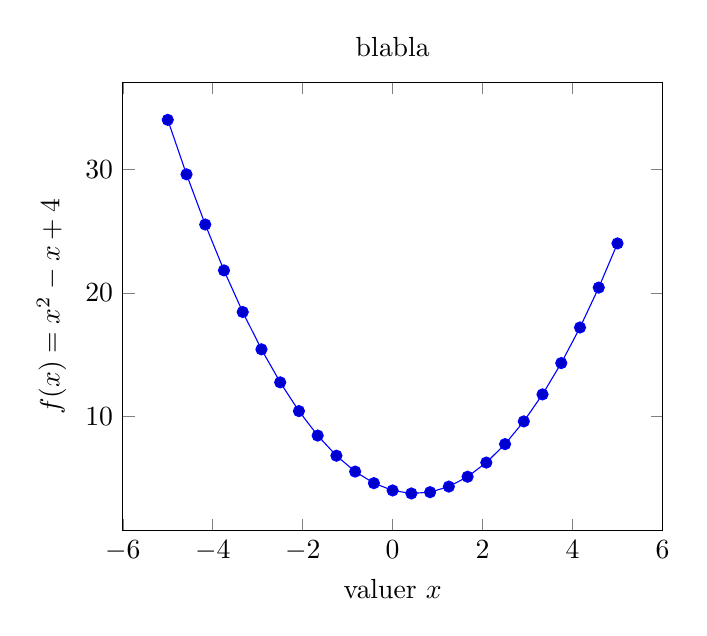
\begin{tikzpicture}
        \begin{axis}[ 
        title={blabla},
        xlabel={valuer $x$},
        ylabel={$f(x) = x^2 - x +4$}
        ] 
        \addplot {x^2 - x +4}; 
        \end{axis}
        \end{tikzpicture}
       %\vspace{2cm}
        \begin{tikzpicture}
        \begin{axis}
        \addplot[color=red]{exp(x)};
        \end{axis}
        \end{tikzpicture}
        
        }
    
  
 % ------------------------------------ PARTIE 5------------
        \block{\textsc{Partie 5}}{\lipsum[1]  
        
        \input{table/table} 
            \vspace{-2cm}}

 
 %%%%%%%%%%%%%%%%%%%%%%%% Column 3 %%%%%%%%%%%%%%%%%%%%%%%%%   
    \subcolumn{.33}

    % ---------------------------------------------
        \block{\textsc{Conclusion}}{
        \lipsum[1]
        
        \vspace{0.5cm}
        \lipsum[2] \cite{ref1}
        \vspace{0.5cm}}

    % ----------------------------------------------
        \block{}{
        \vspace{3cm}
            \textbf{SPA}: Société Protectrice des Animaux $\bullet$
            \textbf{CAF}: Caisse d'Allocations Familiales $\bullet$
            \textbf{WER}: Word Error Rate }   
    
    \end{subcolumns}
    

    % ---------------------------------  References ----------
    \block{}{\vspace{1cm}
       \printbibliography}
       \end{columns}

% ----------------- Footer -------------
\node [above right, text=white,outer sep=45pt,minimum width=\paperwidth, align=center, draw, fill=titledarkcolor, color=Orange] at (-43.6,-61) { \textcolor{white}{\normalsize Contact: prenom.nom@univ-lyon2.fr}};

\end{document}
